%----------------------------------------------------------------------------------------
%	PACKAGES AND DOCUMENT CONFIGURATIONS
%----------------------------------------------------------------------------------------

\documentclass[10pt,a4paper]{article}
\usepackage[utf8]{inputenc}
\usepackage{graphicx} % Required for the inclusion of images
\graphicspath{{res/}}
\usepackage{natbib} % Required to change bibliography style to APA
\usepackage{amsmath} % Required for some math elements 
\usepackage{amsfonts}
\usepackage{amssymb}
\usepackage[T1,T2A]{fontenc}

\setlength\parindent{0pt} % Removes all indentation from paragraphs

\renewcommand{\labelenumi}{\alph{enumi}.} % Make numbering in the enumerate environment by letter rather than number (e.g. section 6)

%----------------------------------------------------------------------------------------
%	DOCUMENT INFORMATION
%----------------------------------------------------------------------------------------

\title{GnuPG} % Title

\author{Виктор \textsc{Борисов}} % Author name

\date{\today} % Date for the report

\begin{document}

\maketitle % Insert the title, author and date

\newpage

\tableofcontents

\newpage

%----------------------------------------------------------------------------------------
%	SECTION 1
%----------------------------------------------------------------------------------------

\section{Цель работы}

Научиться создавать сертификаты, шифровать файлы и ставить ЭЦП.
 
%----------------------------------------------------------------------------------------
%	SECTION 2
%----------------------------------------------------------------------------------------

\section{Ход работы}

\subsection{Kleopatra}
\label{kleopatra}

- это графический интерфейс для GPG. Для ОС Windows доступен с пакетом Gpg4win.

Пользовательский интерфейс с созданной ключевой парой представлен на рисунке \ref{fig:kleopatra_gui}


\begin{figure}[h]
\begin{center}
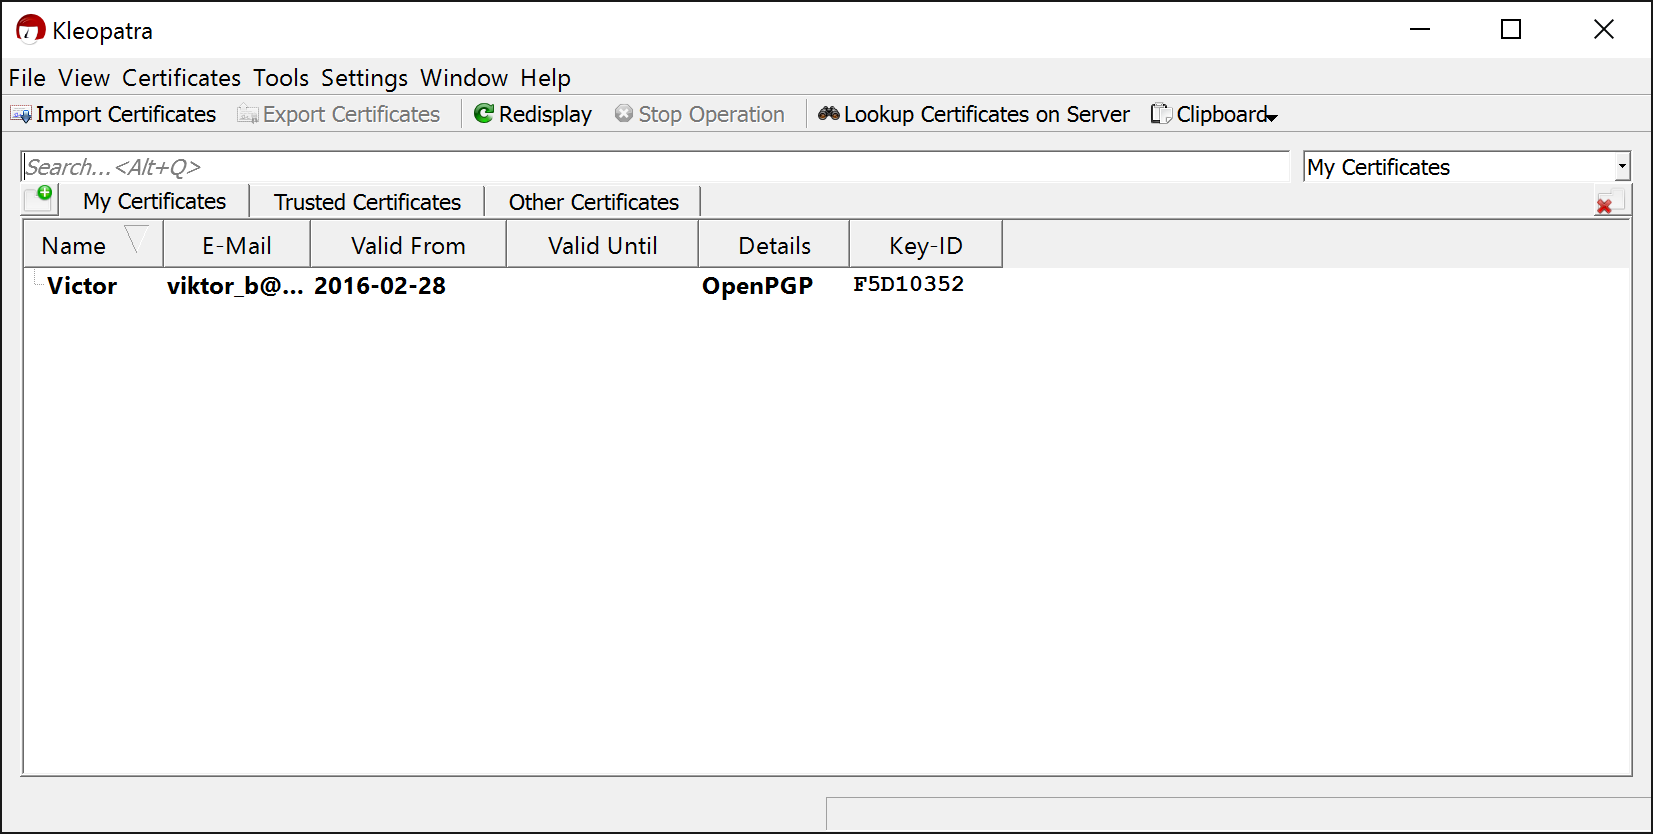
\includegraphics[width=0.65\textwidth]{kleopatra_gui} % Include the image placeholder.png
\caption{Пользовательский интерфейс Kleopatra.}
\label{fig:kleopatra_gui}
\end{center}
\end{figure}


\subsection{Экспорт сертификата}
\label{cert_export}

Экспорт сертификата в файл (File -> Export Certificate) *.asc
Содержание файла представлено на рисунке \ref{fig:cert_exported}

\begin{figure}[h]
\begin{center}
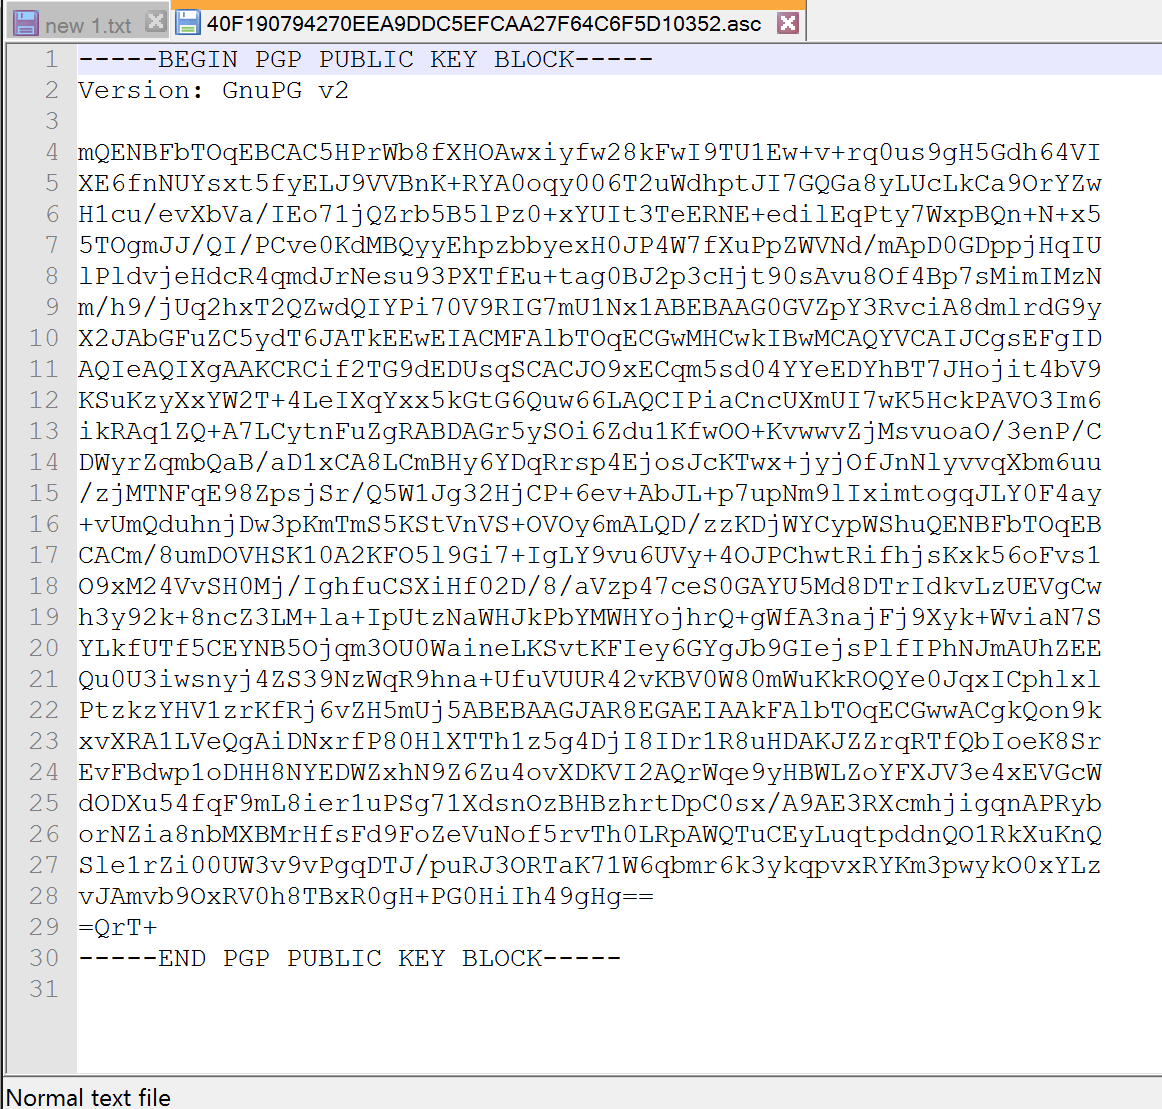
\includegraphics[width=0.5\textwidth]{cert_exported} % Include the image placeholder.png
\caption{Экспорт сертификата.}
\label{fig:cert_exported}
\end{center}
\end{figure}

\subsection{ЭЦП}
\label{echp}

Поставлена ЭЦП на файл (File -> Sign/Encrypt Files).
Шаги процесса отображены на Рисунках \ref{fig:encrypt_1}, \ref{fig:encrypt_3}


\begin{figure}[h]
\begin{center}
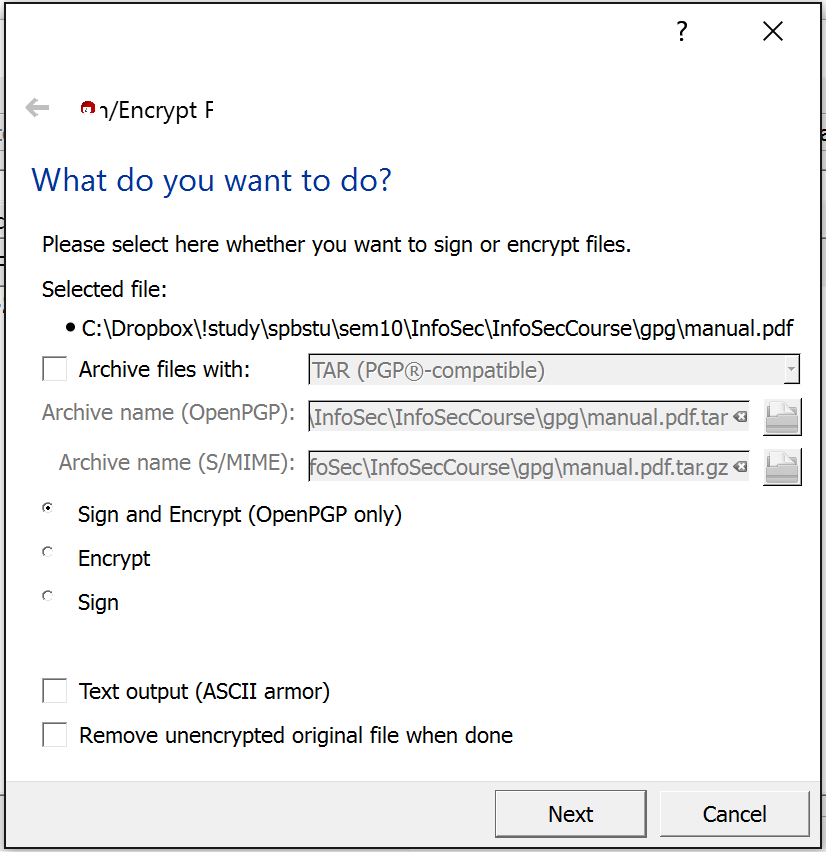
\includegraphics[width=0.4\textwidth]{encrypt_1} % Include the image placeholder.png
\caption{Файл для подписи}
\label{fig:encrypt_1}
\end{center}
\end{figure}
\begin{figure}[h]
\begin{minipage}[h]{0.4\textwidth}
\center{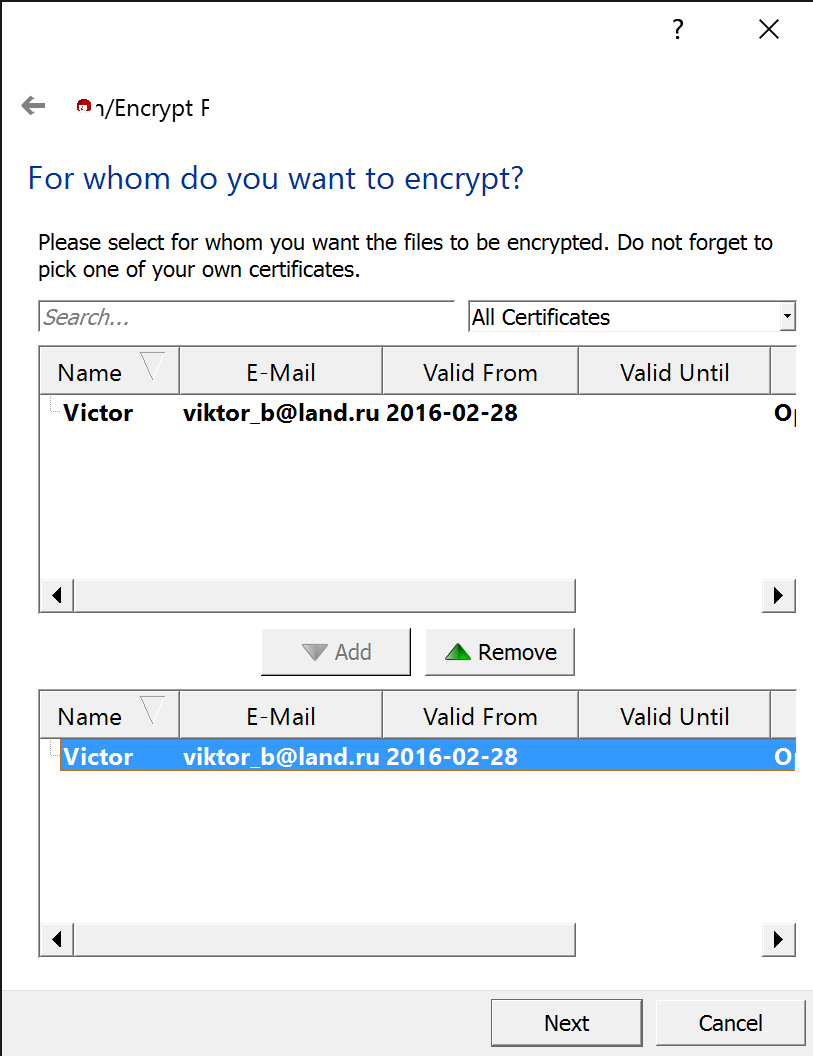
\includegraphics[width=1\textwidth]{encrypt_2}}
\end{minipage}
\hfill
\begin{minipage}[h]{0.4\textwidth}
\center{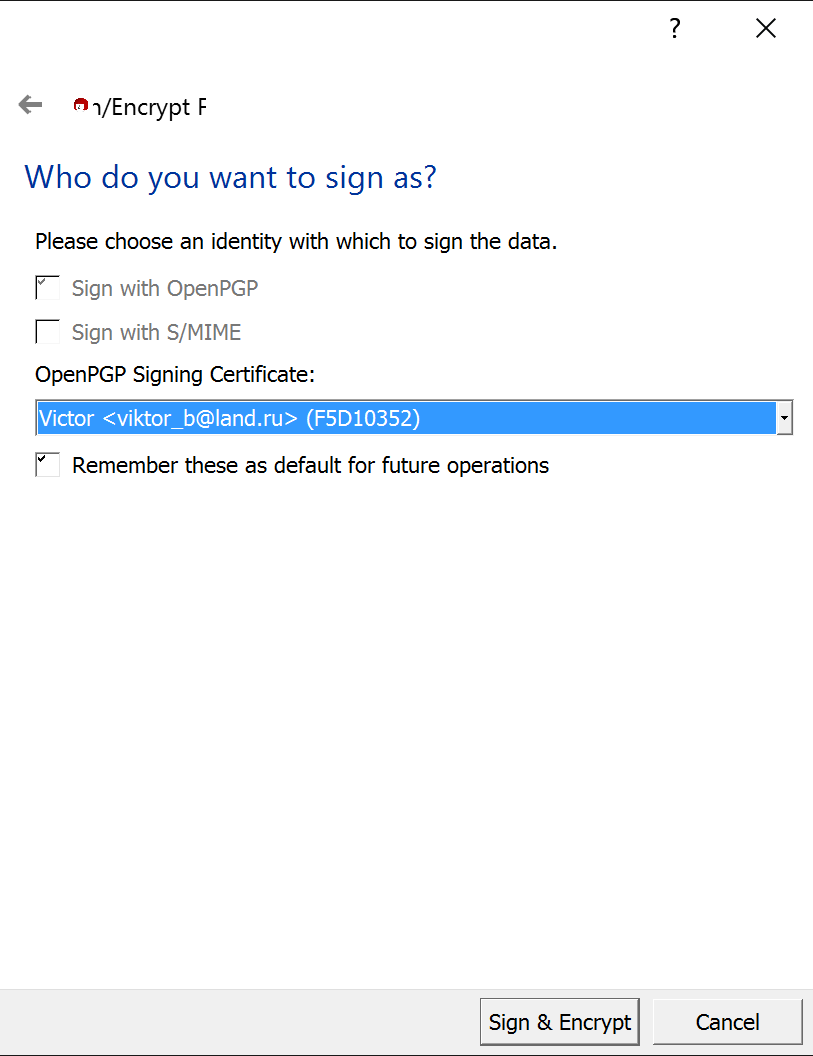
\includegraphics[width=1\textwidth]{encrypt_3}}
\end{minipage}
\caption{Выбор сертификатов}
\label{fig:encrypt_3}
\end{figure}

\subsection{Работа с GPG средствами командной строки}
\label{gpg_console}

Операции, проделанные с помощью графического интерфейса Kleopatra, можно повторить использую лишь консоль.

Создание нового ключа производится с помощью команды (Рисунок \ref{fig:console_create_1}, \ref{fig:console_create_2})
\begin{verbatim}
gpg --gen-key
\end{verbatim}

\begin{figure}[h]
\begin{center}
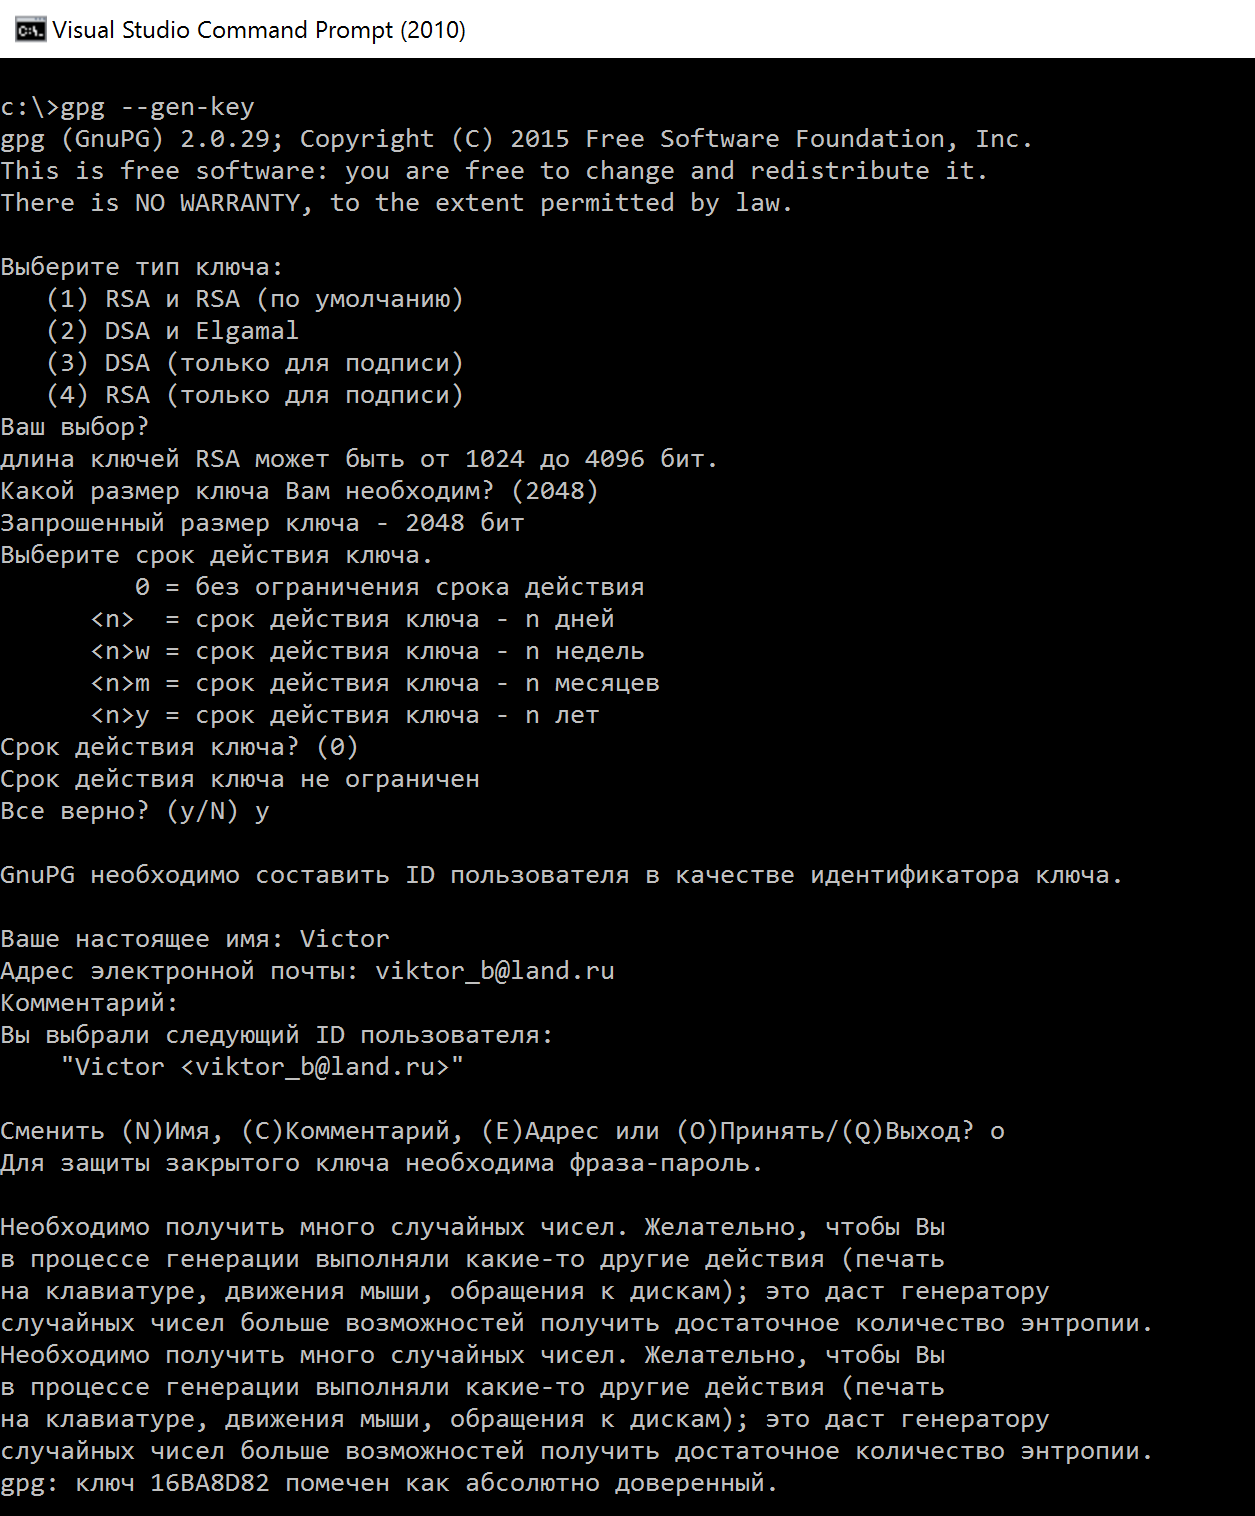
\includegraphics[width=0.5\textwidth]{console_create_1} % Include the image placeholder.png
\caption{Создание ключа.}
\label{fig:console_create_1}
\end{center}
\end{figure}

\begin{figure}[h]
\begin{center}
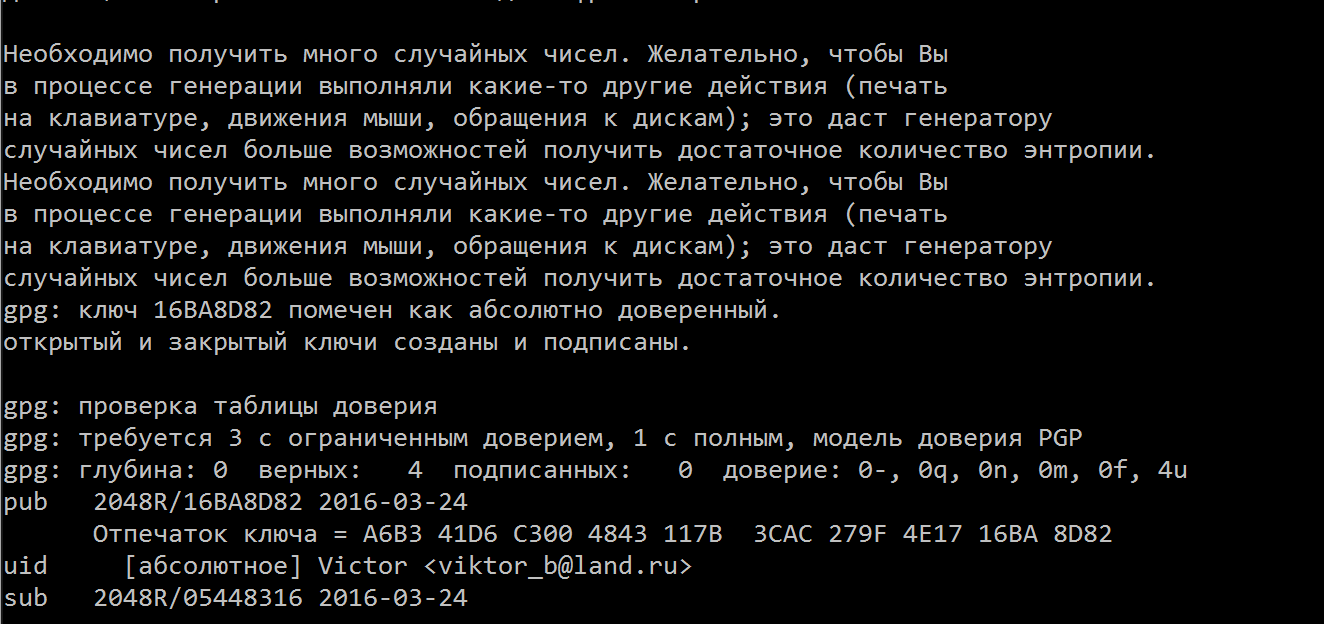
\includegraphics[width=0.5\textwidth]{console_create_2} % Include the image placeholder.png
\caption{Создание ключа.}
\label{fig:console_create_2}
\end{center}
\end{figure}

Для просмотра имеющихся в системе ключей необходимо воспользоваться командой (список ключей отображен на Рисунке \ref{fig:console_list})
\begin{verbatim}
gpg --list-keys
\end{verbatim}


\begin{figure}[h!]
\begin{center}
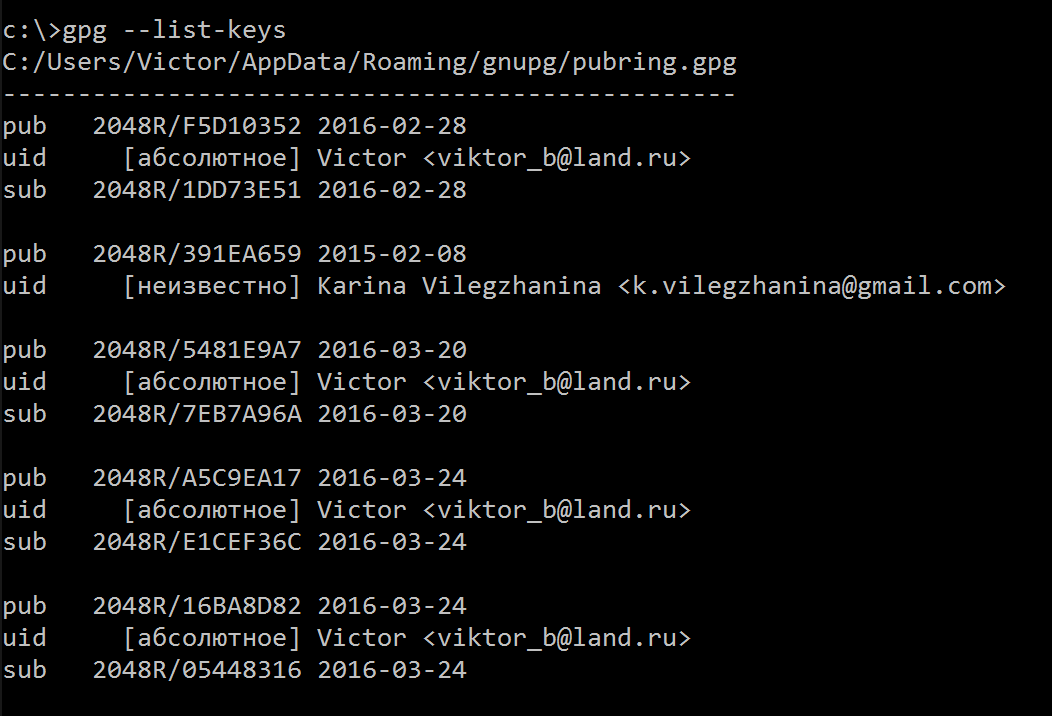
\includegraphics[width=0.5\textwidth]{console_list} % Include the image placeholder.png
\caption{Список ключей.}
\label{fig:console_list}
\end{center}
\end{figure}

Экспорт ключей возможен с помощью команды
\begin{verbatim}
gpg --export
\end{verbatim}
с различными опциями (например, вывод в файл, вид представления, выбор ключа для экспорта).

Для импорта
\begin{verbatim}
gpg --import Имя_файла
\end{verbatim}

\newpage

\section{Вывод}


В ходе работы было изучено средство GPG, позволяющее шифровать и подписывать файлы, проверять электронную подпись


%----------------------------------------------------------------------------------------
%	END
%----------------------------------------------------------------------------------------


\end{document}

